\documentclass{article}
\usepackage[utf8]{inputenc}
\usepackage[landscape]{geometry}

\title{ChristmasTree, NOWAE Gadget 2020 - Idea}
\author{Marco Giammarini}
\date{September 2020}

\usepackage{tikz}
\usetikzlibrary{shapes,arrows,fit,calc}
\tikzset{box/.style={draw, rectangle, rounded corners, thick, node distance=7em, text width=6em, text centered , minimum height=3.5em}}
\tikzset{container/.style={draw, rectangle, dashed, inner sep=1em}}
\tikzset{line/.style={draw, thick, -latex}}
\tikzset{power/.style={draw, color=red, ultra thick, -latex}}

\begin{document}
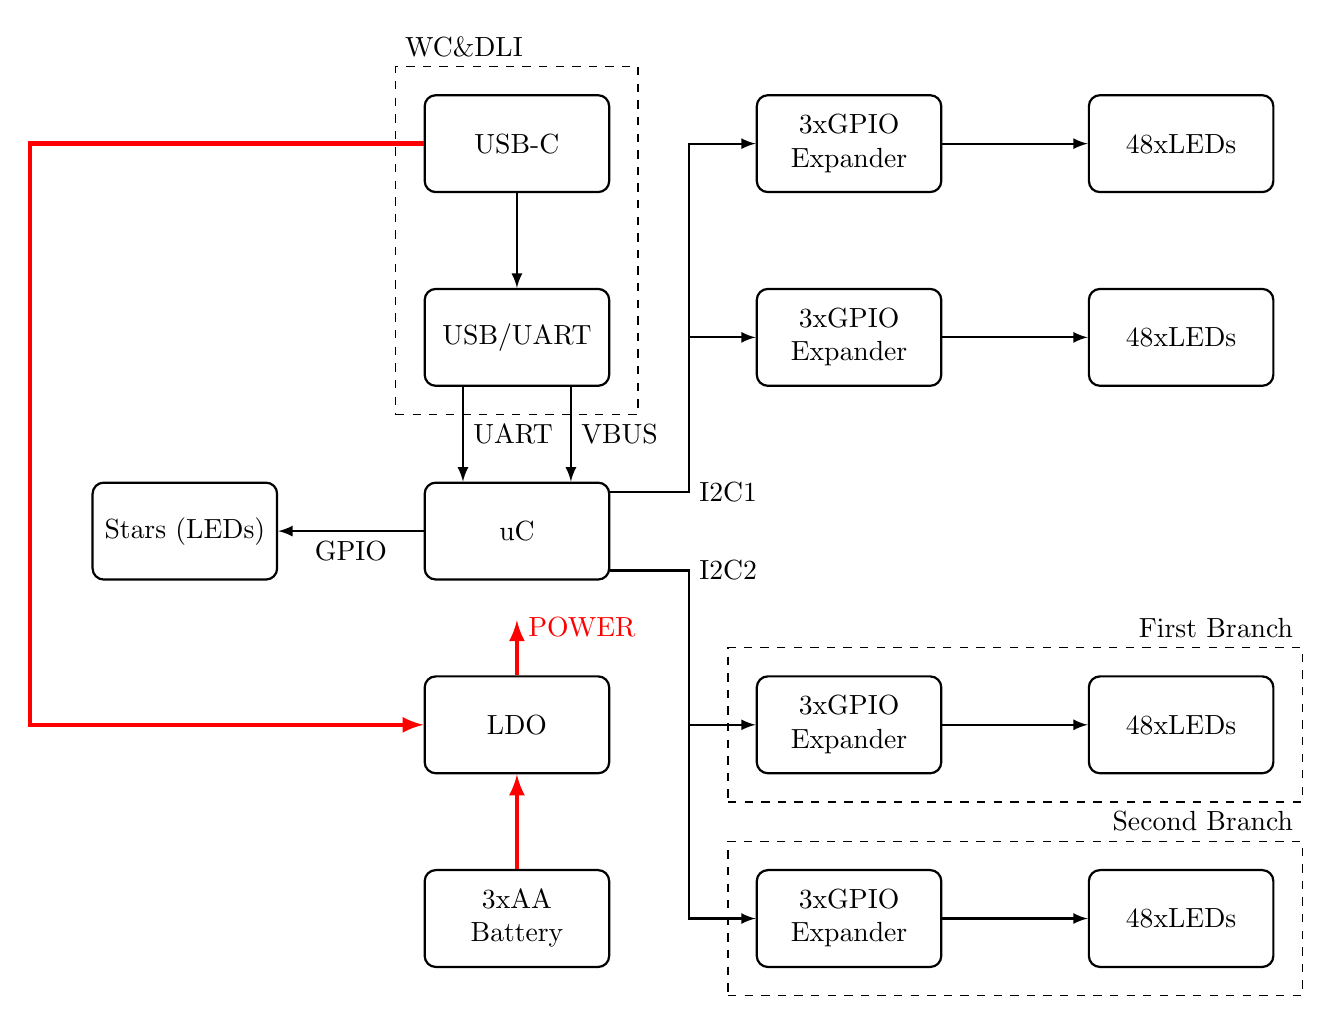
\begin{tikzpicture}[auto]

\node [box] (mcu) {uC};
\node [box, below of=mcu] (ldo) {LDO};
\node [box, below of=ldo] (battery) {3xAA Battery};
\node [box, above of=mcu] (ftdi) {USB/UART};
\node [box, above of=ftdi] (usb) {USB-C};

\node [box, left of=mcu, node distance=12em] (star) {Stars (LEDs)};

\node [box, right of=ftdi, node distance=12em] (gpio1) {3xGPIO Expander};
\node [box, right of=gpio1, node distance=12em] (light1) {48xLEDs};
\node [box, right of=usb, node distance=12em] (gpio2) {3xGPIO Expander};
\node [box, right of=gpio2, node distance=12em] (light2) {48xLEDs};

\node [box, right of=ldo, node distance=12em] (gpio3) {3xGPIO Expander};
\node [box, right of=gpio3, node distance=12em] (light3) {48xLEDs};
\node[container , fit=(gpio3) (light3)] (board1) {};
\node at (board1.north east) [above left,node distance=0 and 0] {First Branch};
\node [box, right of=battery, node distance=12em] (gpio4) {3xGPIO Expander};
\node [box, right of=gpio4, node distance=12em] (light4) {48xLEDs};
\node[container , fit=(gpio4) (light4)] (board2) {};
\node at (board2.north east) [above left,node distance=0 and 0] {Second Branch};

\node[container , fit=(usb) (ftdi)] (debug) {};
\node at (debug.north west) [above right,node distance=0 and 0] {WC\&DLI};

%POWER PATH
\path [power] (battery) -- (ldo);
\path [power] (usb.west) -- ($(usb.west)-(5,0)$) -- ($(ldo.west)-(5,0)$) -- (ldo.west);
\path [power] (ldo.north) -- node [above right] {POWER} ($(ldo.north)+(0,0.7)$);

%GPIO LINE
\path [line] (mcu) -- node {GPIO} (star);

%USB
\path [line] (usb) -- (ftdi);
\path [line] ($(ftdi.south west)+(0.5,0)$) -- node {UART} ($(mcu.north west)+(0.5,0)$);
\path [line] ($(ftdi.south east)-(0.5,0)$) -- node {VBUS} ($(mcu.north east)-(0.5,0)$);

%I2C TO GPIO EXPANDER
\path [line] ($(mcu.east)+(0,0.5)$) -- ($(mcu.east)+(1.0,0.5)$) node [right] {I2C1} |- (gpio1.west);
\path [line] ($(mcu.east)+(0,0.5)$) -- ($(mcu.east)+(1.0,0.5)$) |- (gpio2.west);

\path [line] ($(mcu.east)+(0,-0.5)$) -- ($(mcu.east)+(1.0,-0.5)$) node [right] {I2C2} |- (gpio3.west);
\path [line] ($(mcu.east)+(0,-0.5)$) -- ($(mcu.east)+(1.0,-0.5)$) |- (gpio4.west);

%GPIO EXPANDER TO LEDS
\path [line] (gpio1) -- (light1);
\path [line] (gpio2) -- (light2);
\path [line] (gpio3) -- (light3);
\path [line] (gpio4) -- (light4);

\end{tikzpicture}

\end{document}